\documentclass[]{UCD_CS_FYP_Report}
% Use scalable fonts and Unicode mappings for searchable, copyable PDF text.
\usepackage{lmodern}
\input{glyphtounicode}
\pdfgentounicode=1
\usepackage{graphicx}
\graphicspath{{Images/}}
\usepackage{listings}
\usepackage{hyperref}

\usepackage{framed}
\usepackage{xcolor}


\renewenvironment{leftbar}{%
    \def\FrameCommand{%
        {\color{gray}\vrule width 1pt}%
        \hspace{12pt}%
    }%
    \MakeFramed{%
        \advance\hsize-\width
        \FrameRestore
        \setlength{\parskip}{0pt}%
    }%
    \itshape
    \vspace{8pt}%
}{%
    \par\vspace{8pt}%
    \endMakeFramed
    \vspace{-\parskip}%
}

\usepackage{tcolorbox}

\newtcbox{\codepill}{
    on line,
    colback=gray!12,
    colframe=gray!12,
    boxrule=0pt,
    arc=3pt,
    boxsep=2pt,
    left=2pt,
    right=2pt,
    top=0.5pt,
    bottom=0.5pt,
    fontupper=\ttfamily\fontsize{9}{9}\selectfont
}

\hypersetup{
    colorlinks=true,
    linkcolor=blue,
    filecolor=magenta,      
    urlcolor=cyan,
}
\lstset{
    mathescape=true,
    basicstyle = \ttfamily,
    keywordstyle=\color{blue!70!black}\bfseries,
    commentstyle=\color{green!40!black}\itshape,
    stringstyle=\color{orange!70!black}
}
%\usepackage[backend=biber,style=chicago-authordate]{biblatex}
\usepackage[backend=biber,style=nature]{biblatex}
\renewcommand*{\mkbibacro}[1]{#1}
\addbibresource{references.bib}

\usepackage{minted}
\usepackage{csquotes}
\DeclareQuoteStyle{straight}{\textquotedbl}{\textquotedbl}{\textquotesingle}{\textquotesingle}
\setquotestyle{straight}

\DeclareMathSizes{11}{11}{8}{5}

\usepackage{enumitem}
\setlist[itemize]{itemsep=0pt, parsep=0pt}

%%%%%%%%%%%%%%%%%%%%%%
%%% Input project details

\def\studentname{Ewan Sheridan}% Edit with your name
\def\studentid{23336833}% Edit with your student id
\def\projecttitle{Simulation \& Scheduling of Parallelisable Tasks Across Local Devices and MEC Infrastructure 
} % Edit with you project title
\def\supervisorname{Professor Liam Murphy}


\begin{document}
\maketitle

%%%%%%%%%%%%%%%%%%%%%%
%%% Table of Content

\tableofcontents
%\pdfbookmark[0]{Table of Contents}{toc}\newpage
%\newpage


%%%%%%%%%%%%%%%%%%%%%%
%%% Your Abstract here
\abstract
The computational power of laptops, smartphones and other user devices has improved dramatically in recent years. The cloud computing paradigm was first introduced to allow users to execute large computations by performing said computations on servers in datacentres. This meant that large problems could be computed in an acceptable time, but for smaller problems, the network overhead of offloading to the cloud was non-negligible. Multi-access edge computing brought slightly less powerful machines geographically closer to users, which decreased RTTs considerably and improved the overall latency of task completion. 

This project poses the question: \textit{What if some of the computation could be done on the local device itself?} To completely eliminate edge and cloud offloading would be impractical for large tasks, so in this project tasks are divided into subtasks that can run in parallel. A scheduling algorithm divides these subtasks into three groups to run on the cloud, the edge cluster, and the local device itself.

To facilitate the development and testing of this algorithm, a simulator is also developed using the \textit{SimPy} Python framework. The creation of this simulator and the implementation of the local-device-aware parallel scheduling algorithm form the main body of work for this project.


%%%%%%%%
\chapter{Project Specification}
\textbf{Mandatory}
\vspace{-1.5em}
\begin{itemize}
    \item Literature review of task scheduling, offloading, parallelism in MEC, and use of local devices as part of a MEC system
    \item Review of previous FYPs in the same area (Cian Boyle, James Finn, Luke King)
    \item Simple implementation of a MEC simulator with three basic levels (cloud, edge, local device) alongside a central scheduler for parallelisable tasks
    \item Verification and validation that the simulator works properly (e.g. a 100 MI subtask takes 1 second on a 100 MIPS processor, and other similar tests)
    \item A basic first implementation of a scheduling algorithm in the simulator with fixed parameters and a small number of devices and homogeneous subtasks
\end{itemize}
\vspace{-0.5em}

\textbf{Discretionary}
\vspace{-1.5em}
\begin{itemize}
    \item Improvement to the algorithm to consider more users
    \item Extension of the simulator to allow for more flexibility e.g. different processing speeds i.e. heterogeneous processors, multiple tasks per user, etc.
    \item Adaptation of the algorithm to work under dynamically changing conditions
\end{itemize}
\vspace{-0.5em}

\textbf{Exceptional}
\vspace{-1.5em}
\begin{itemize}
    \item Enhanced algorithm that considers parallelisable tasks of a more complex nature, for
example, heterogeneous subtasks or dependencies between subtasks
\end{itemize}

%%%%%%%%
\chapter{Introduction}
The \textit{Multi-access Edge Computing} paradigm can be described as being made up of three layers (see Figure \ref{fig:mec}). The first of these layers is the \textit{Cloud}, where computation can be done fastest, but its network (and physical) distance from the user results in long round-trip times (RTTs). The middle layer, the \textit{Edge}, aims to mitigate the RTT issue by being situated much closer to the user. 

However, the servers at the edge are much less powerful than those at the cloud. This means that for any given task there is a trade-off decision to be made: compute the task quickly at the cloud but suffer a long propagation delay, or leverage the lower network latency of the edge but compromise on slower computation speed.

This decision problem is one of the main motivators of research in the area of MEC scheduling. However, it fails to consider that the third layer, the \textit{User}, is also capable of computation. User devices like smartphones and laptops are often ignored in MEC scheduling, but this decade has seen a 


\vspace{4em}
\textit{Introduce your vision of the project here. Describe the domain of the project, and the intended application. A well-written report will answer three key questions: What am I doing in this project? Why is it worth doing? How do I plan to go about it? In this introductory section, offer a concise answer to the What, and follow-up with a compelling account of the Why. Leave the How to a subsequent section. Do not try to do too much in any single section of the report. By providing details in a logical order, you will show that you have a plan for the report and the project.}

%%%%%%%%
\chapter{Related Work and Ideas}
Much research has been carried out in the fields and areas that are relevant to this project. This chapter outlines literature in the area of cloud computing, and subsequently the motivation for edge computing and MEC. A comparison of the existing ways to simulate a MEC environment is outlined, with reference to past UCD final year projects, followed by a review of different approaches to the scheduling of parallelisable tasks, not only in MEC systems but in general. Finally, research relating to the offloading of tasks due to local constraints is detailed.

\section{Cloud Computing}
The National Institute of Standards and Technology (NIST) \cite{mell2011nist} defines cloud computing as follows:

\begin{leftbar}
    Cloud computing is a model for enabling ubiquitous, convenient, on-demand network access to a shared pool of configurable computing resources (e.g., networks, servers, storage, applications, and services) that can be rapidly provisioned and released with minimal management effort or service provider interaction. 
\end{leftbar}

A major benefit that cloud computing brings to an organisation is the elasticity with which hardware resources can be provisioned and released \cite{mell2011nist}. An application can harness the powerful computation of large data centre servers without the need to purchase or house it, which is particularly useful when these resources are only needed periodically. 

The pay-as-you-go pricing model is attractive in such cases. Despite costing more per-computation, the overall cost is still less than that of the organisation purchasing and running powerful servers themselves, which could remain under-utilised for long periods \cite{uslu2025cc, fourati2025cloud}. Instead, cloud providers run many servers, dynamically allocating computing resources according to the combined demands of multiple users. Figure \ref{fig:elastic} illustrates that this larger volume allows resources to be allocated much more flexibly, and minimise the amount of wasted energy.

\begin{figure}
    \centering
    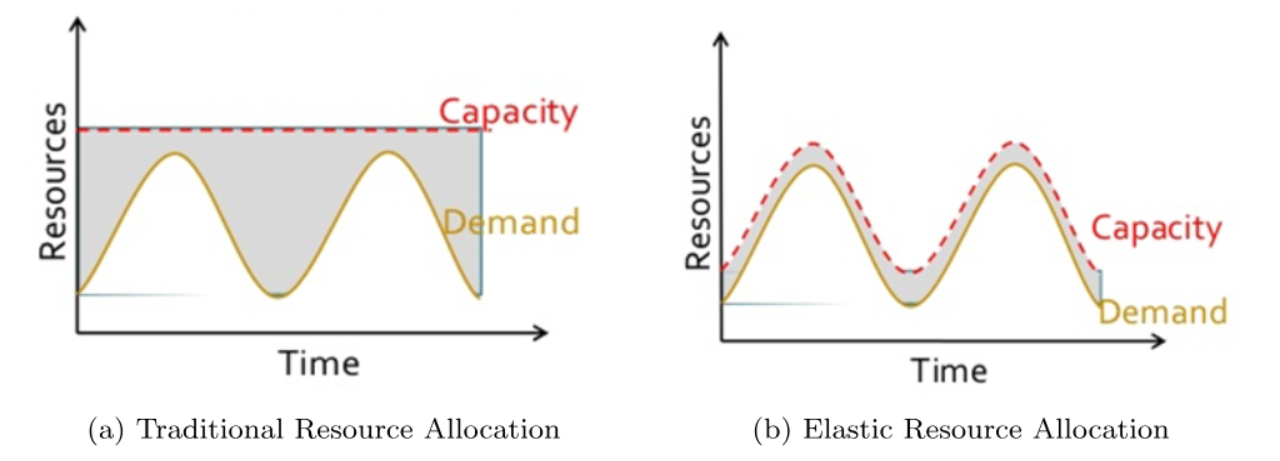
\includegraphics[width=0.75\linewidth]{elastic.png}
    \caption{Having large amounts of resources available can lead to overprovisioning; cloud computing's elasticity combines multiple services so supply can always stay close to demand \cite{fourati2025cloud}}
    \label{fig:elastic}
\end{figure}

In 2014, 17.8\% of EU enterprises were purchasing cloud services; eleven years later, in 2025 the figure was 52.7\% \cite{eurostat2026cloud}. However, for time-sensitive tasks, the physical distance between end users and the cloud, as well as network delays, become bottlenecks which edge computing aims to solve.

\section{Edge Computing}
Edge computing is a paradigm that aims to solve the aforementioned issues in cloud computing. Sometimes referred to as \textit{fog computing}, the general idea is that substantial computing resources are placed at the \enquote{edge} of the Internet, close (in terms of physical distance and/or low latency) to the end users \cite{hong2024edge}, as can be seen in Figure \ref{fig:edge}. An edge server can process both \textit{downstream data} (originating from cloud services) and \textit{upstream data} (originating from end devices). 

\begin{figure}
    \centering
    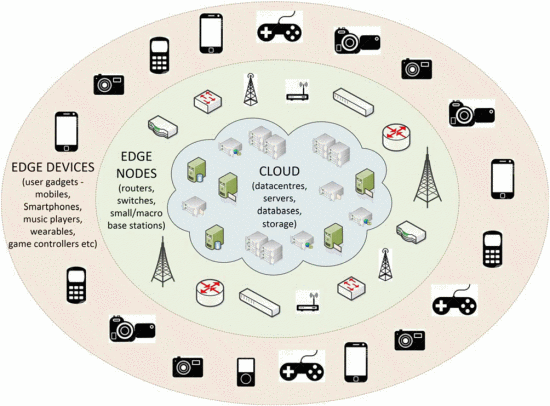
\includegraphics[width=0.5\linewidth]{edge.png}
    \caption{Edge devices and edge nodes (or \enquote{edge servers}) in relation to the cloud \cite{varghese2016edge}}
    \label{fig:edge}
\end{figure}

The decrease in network delay, primarily due to a decrease in physical distance or the number of network hops, is a primary benefit of edge computing. For small tasks, computing them at the edge can be significantly faster (overall) than computing at the cloud. However, unlike traditional cloud computing, a typical edge server cluster is significantly less powerful \cite{mann2021fog} and may increase task execution time for computationally expensive tasks. Because of this, the overall completion time of processing a large task can still be faster on the cloud, despite its longer round-trip time (RTT). This trade-off, and deciding which tasks get done at the edge, versus which get done on the cloud, is a central research problem in edge computing \cite{avan2023sched}.


\section{Multi-access Edge Computing (MEC)}
Previously known as \textit{Mobile Edge Computing} \cite{etsi2016mec}, multi-access edge computing is one specific implementation of the edge computing paradigm. It places edge servers within mobile and wireless access networks. Typically, a MEC system can be conceptually thought of as being made up of three layers: user devices (e.g. mobile phones) at the \enquote{edge} of the system, edge servers at a base station or access point, and the central cloud server at the \enquote{core} \cite{Abbas2018MEC}. 

Although some implementations have the middle layer consisting of multiple sub-layers and \textit{proxy servers} \cite{lee2018complexmec, yu2023proxy}, this project adopts a simpler structure as seen in Figure \ref{fig:mec}. This abstraction allows focus to be directed at the scheduling of tasks across the three layers, rather than explicitly modelling low-level networking infrastructure that otherwise can be defined by a simple parameter. The idea that an edge server's RTT will be much lower than the cloud's, combined with the cloud's greater computational power, creates the central scheduling problem that motivates this project.

\begin{figure}
    \centering
    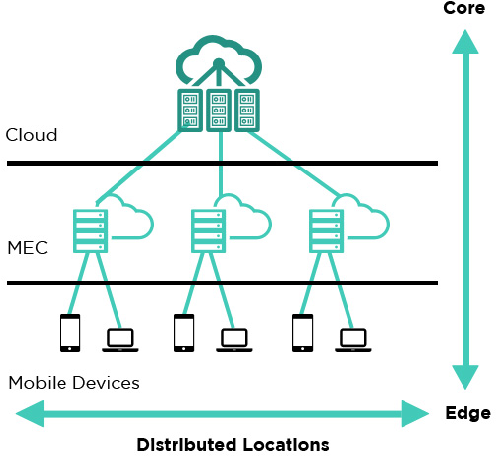
\includegraphics[width=0.5\linewidth]{mec.png}
    \caption{A simplified three-layer MEC architecture \cite{Abbas2018MEC}}
    \label{fig:mec}
\end{figure}

\section{Existing MEC Simulators}
MEC presents a wide range of research challenges, including (but certainly not limited to) task scheduling, as will be investigated by this project. To test or verify a solution to a MEC problem, simulation of that problem's processes is a necessity. One useful paper for this section was Kunde et al.'s \enquote{Comparison of simulators for fog computing} \cite{kunde2020comp}. There is a collection of simulators and frameworks that are specifically for MEC. In the past, UCD final year projects in this area have tended to use the \textit{iFogSim} simulator, or its successor \textit{iFogSim2}.

\subsection{iFogSim2} \label{iFogSim2}
With \textit{CloudSim} and \textit{iFogSim} as its so-called progenitors, \textit{iFogSim2} \cite{ifogsim} was built by the same group of researchers in Melbourne that first developed the original \textit{CloudSim}. It describes itself as:

\begin{leftbar}
    A Toolkit for Modeling and Simulation of Resource Management Techniques in Internet of Things, Edge and Fog Computing Environments
\end{leftbar}

\begin{figure}
    \centering
    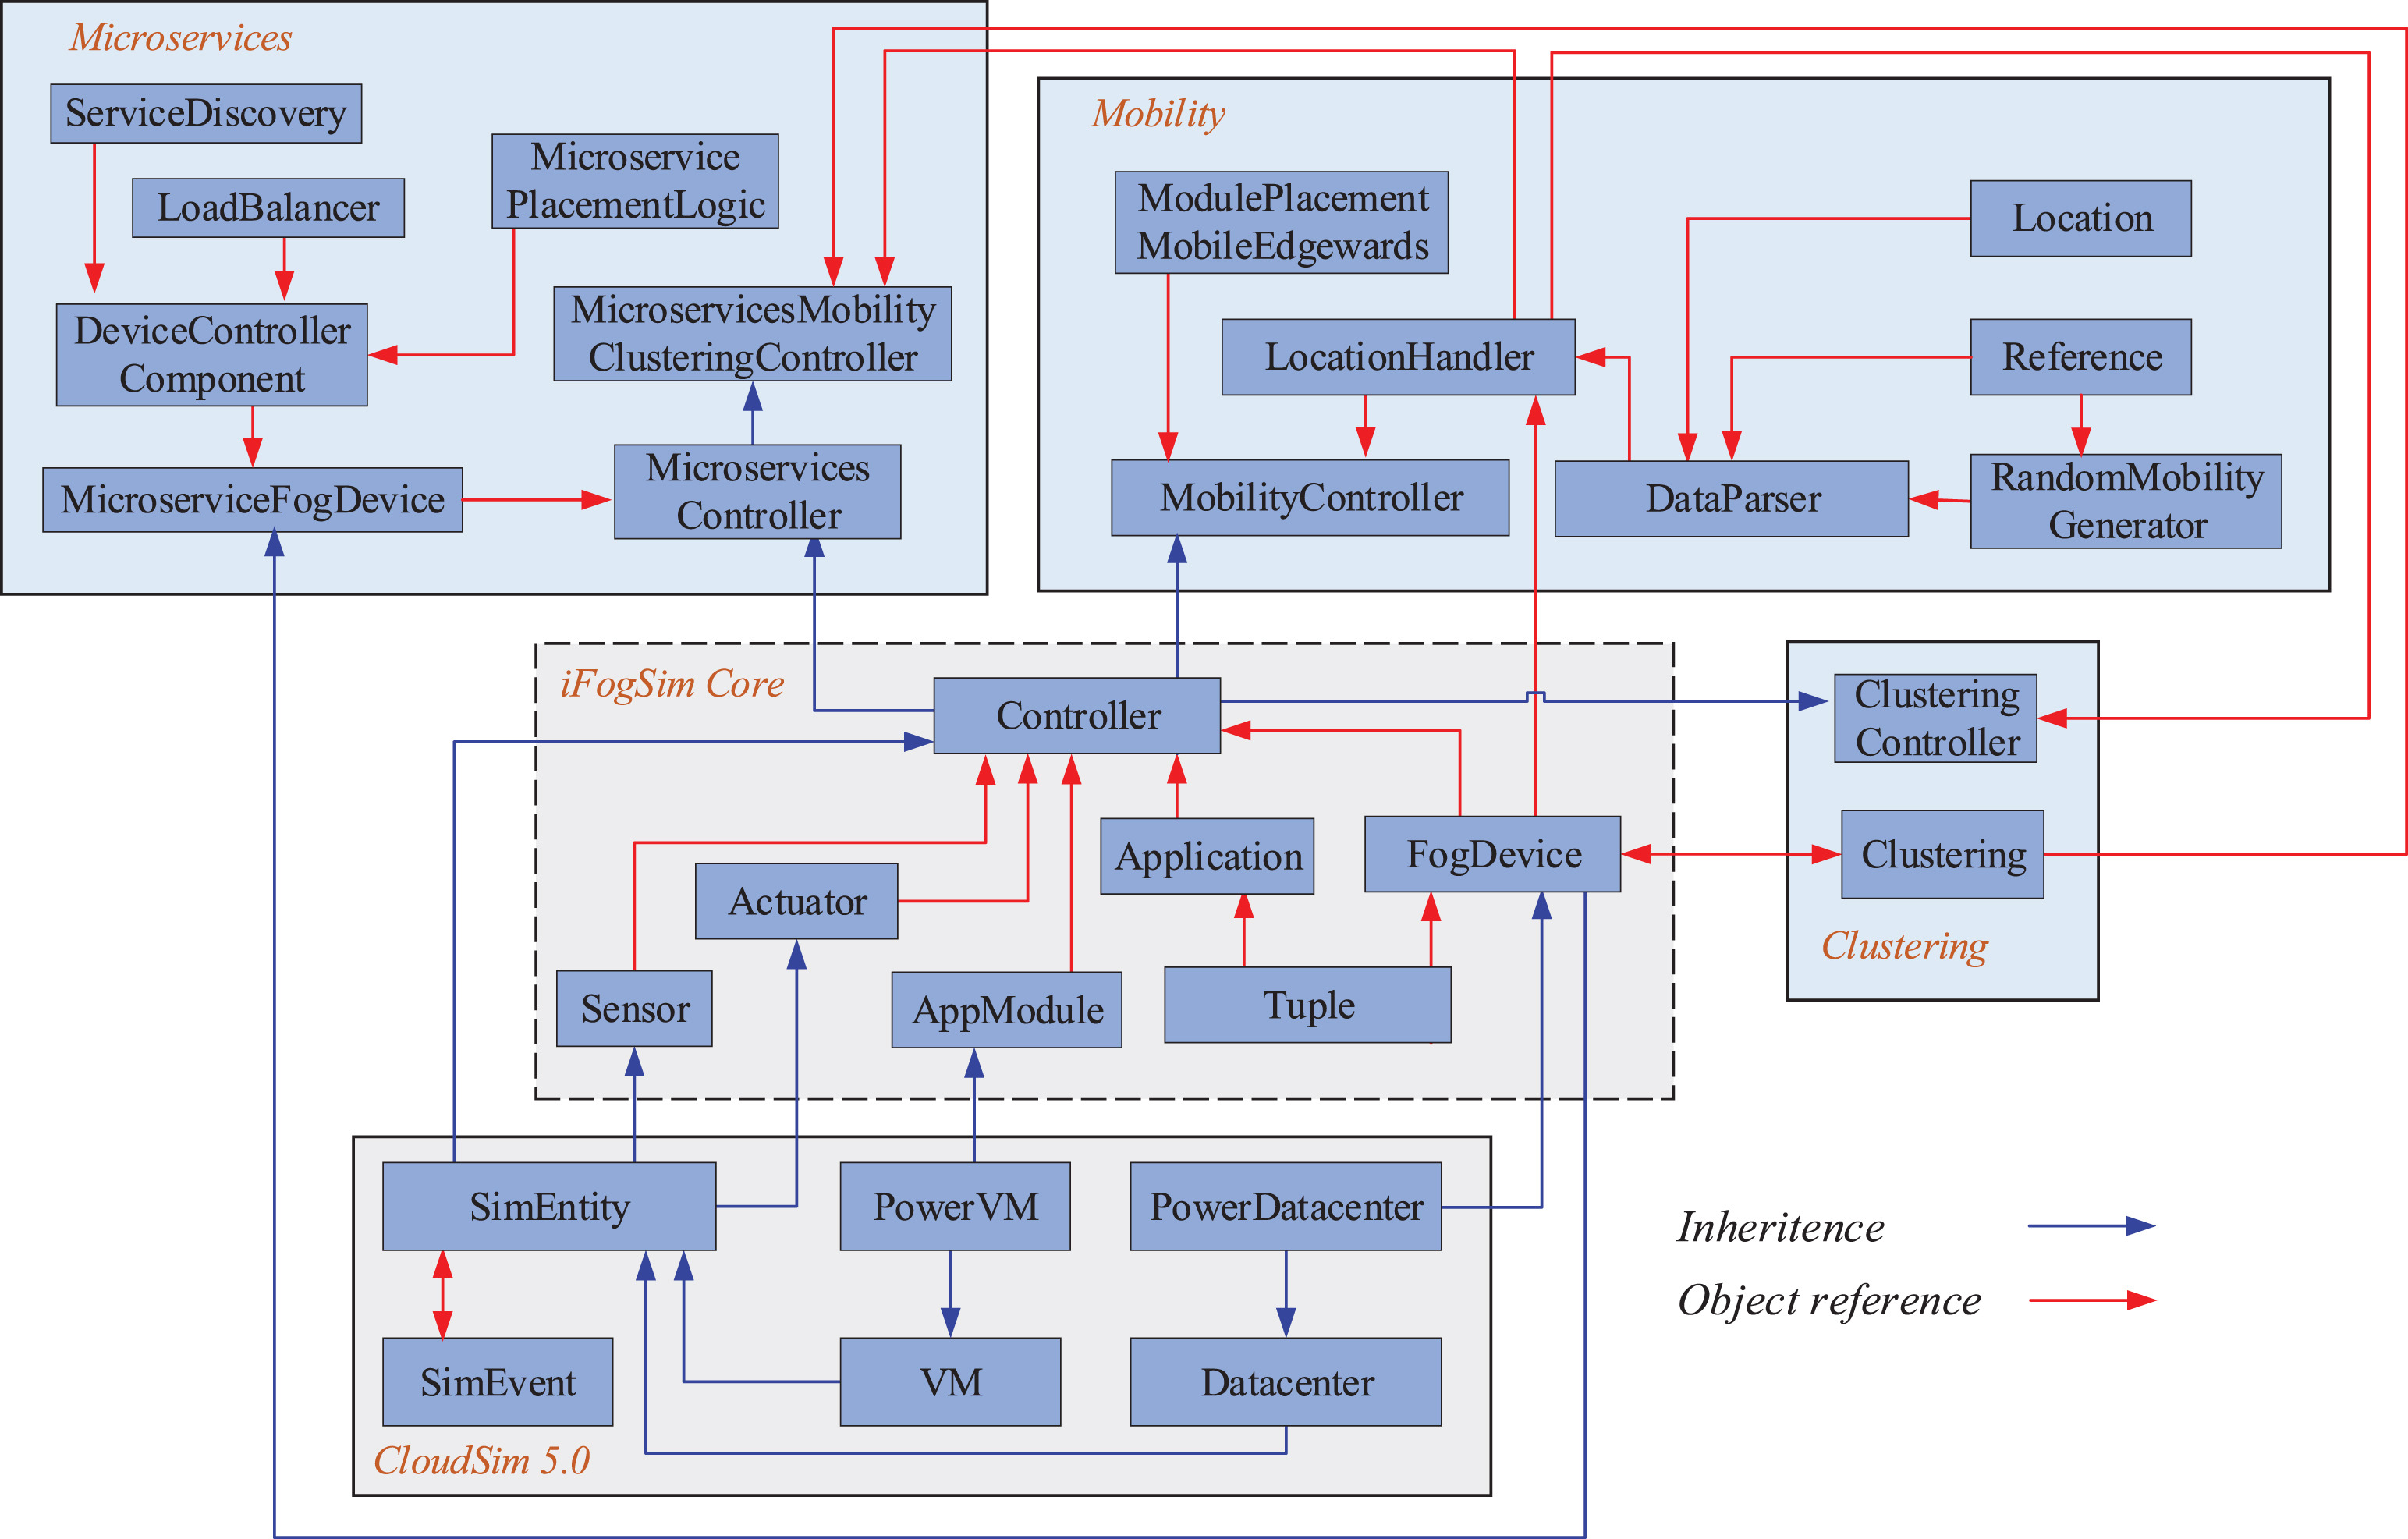
\includegraphics[width=0.75\linewidth]{ifogsim.png}
    \caption{Class diagram of iFogSim2, illustrating its architecture \cite{ifogsim}}
    \label{fig:ifogsimarch}
\end{figure}

Written in Java, the simulator offers a breadth of pre-defined classes to build a fog computing environment from. Its vast array of potential use-cases comes with the caveat of a steep learning curve, and a tendency to produce errors and bugs. On the former, one would expect an object-oriented edge computing simulator to come pre-packaged with simple classes that intuitively map to the real world entities within a MEC system, for example, classes like \codepill{EdgeServer}, \codepill{CloudServer}, \codepill{Task}, \codepill{Scheduler}, etc. that would have constructors requiring very few arguments. Instead, most classes have constructors requiring numerous parameters, including those unrelated to the intended simulation. Some parameters are often themselves objects that need instantiation. For example:
\vspace{-0.75em}
\begin{minted}{java}
FogDevice(String name, FogDeviceCharacteristics characteristics,
    VmAllocationPolicy vmAllocationPolicy, List<Storage> storageList, 
    double schedulingInterval, double uplinkBandwidth, 
    double downlinkBandwidth, double uplinkLatency, double ratePerMips)

FogDeviceCharacteristics(String architecture, String os, String vmm,
    final Host host, double timeZone, double costPerSec, double costPerMem,
    double costPerStorage, double costPerBw)
\end{minted}

To add to this, the meaning of each class in the system is unintuitive, and the hierarchy of the entire system (a substantial portion of which must be understood to create any simulations) is very complex, as can be seen in Figure \ref{fig:ifogsimarch}. The simplest example programs supplied on the official GitHub repository span almost 300 lines of code each. This is in part due to the verbose nature of the Java programming language, but is primarily because of the bloated design of \textit{iFogSim2}.

Since its major update and integration with the original \textit{iFogSim} almost two years ago, the GitHub repository containing the source code for the simulator (the primary way to download the software and use it) has not received any updates. Previous students who used \textit{iFogSim2} for their final year projects encountered major bugs that served as large obstacles in their project, diverting development effort away from the novel aspects of their projects. One example is James Finn:

\begin{leftbar}
    The default migration process in iFogSim2 contains several logical limitations in how microservices are handled when users experience mobility events. [...] These issues can result in an incorrect system state where users do not have access to the necessary microservices; therefore, tuples may fail to complete the intended processing loop and prevent the application from executing correctly. \cite{finn2026hepa}
\end{leftbar}

In addition to this, Cian Boyle found that the simulator had no way to test different fine-grained scheduling algorithms. The existing \codepill{FogDevice} class was also not compatible with his goals. Because of this, he had to build an extension to the framework before actually implementing and testing his scheduling algorithm.

\begin{leftbar}
    iFogSim’s current implementation includes an inbuilt \textnormal{\codepill{FogDevice}} class which can be used to represent a physical or virtual computing node within a MEC environment. It models complex behaviours relating to microservice placement and mobility which were not necessary for this  study and previous implementations have made it difficult to have fine-grained control over task execution. \cite{boyle2026pats}
\end{leftbar}

In essence, using the \textit{iFogSim2} simulator, at least for problems at the same level of abstraction as this project, will likely result in as much programming as creating a simpler simulator from scratch.

\subsection{EdgeCloudSim}
The \textit{EdgeCloudSim} \cite{edgecloudsim2018} simulator also builds upon the existing \textit{CloudSim} framework. However, unlike \textit{iFogSim2}, it is not made by the original \textit{CloudSim} developers. It was created specifically to address the concept of \textit{mobility} in MEC, which can be described as:

\begin{leftbar}
    A user's movement may result in disconnection from the old cloudlet [edge server] and reconnection to the new cloudlet, bringing additional task migration overhead. \cite{zheng2024mobility}
\end{leftbar}

The creators of \textit{EdgeCloudSim} discuss in their research paper how \textit{iFogSim} failed to properly model mobility in their simulator, something Finn also observed \cite{finn2026hepa}. It is worth noting that this was the motivation for the creation of \textit{EdgeCloudSim} in 2017, but such functionality does now exist in \textit{iFogSim2} \cite{ifogsim}.

\begin{leftbar}
     iFogSim allows the definition of the location of devices getting service from the fog servers. However, this information is static and it is not updated by any mobility model. The network model in iFogSim is over simplistic where a fixed delay is assigned to links ignoring the effect of network load on the operation. \cite{edgecloudsim2017}
\end{leftbar}

Mobility and network modelling are some of the only areas in which \textit{EdgeCloudSim} can be seen as superior to \textit{iFogSim}, and otherwise they share all the same  undesirable qualities (at least for the implementation of this project) as discussed in subsection \ref{iFogSim2}, such as a steep learning curve, an overly complex class hierarchy, and extremely verbose logging. These issues can be seen in the official tutorials for the simulator. The simulators inherit these problems from the original \textit{CloudSim} simulator, which both of them extend. Therefore, the \textit{EdgeCloudSim} simulator is not well suited to this project since it is not related to the issue of mobility.

\subsection{EdgeSimPy} \label{EdgeSimPy}
Unlike the previous two simulators, which extended \textit{CloudSim} using Java, \textit{EdgeSimPy} \cite{edgesimpy2023} instead uses Python. Despite its name, it is not based on the \textit{SimPy} framework (see section \ref{SimPy}), and the two are completely unrelated. The simulator is built on \textit{Mesa}, which is an agent-based modelling (ABM) framework. Simulated entities are represented as \textit{agents}, which interact and update their states as the simulation progresses \cite{mesa}.

\textit{EdgeSimPy} simulates all physical entities in a MEC system, such as the servers, the end users themselves, the network infrastructure, etc. This is useful for some scenarios and allows the simulator to be used for a broad set of research problems. It allows programmers to operate at a level of abstraction significantly higher than previously discussed \textit{CloudSim} based simulators, however, a meaningful amount of the network topology must be explicitly defined by the programmer.

Since the simulator is agent-based (as opposed to a DES, see section \ref{SimPy}), it operates a constantly ticking clock, for example, where one tick corresponds to 1 ms. Then the different parts of the system, such as end users, edge servers, network connections, etc. are all implemented as \textit{agents}. They each complete simulated work, possibly at the same time, for a duration with respect to the global ticking clock.

It provides models of heterogeneous computing infrastructure, network communication, and application services, with support for custom service placement and migration algorithms. This initially makes it a much better candidate than any other simulator. However, the principal focus of this project is the scheduling of parallelisable tasks across local devices, edge servers, and cloud servers. EdgeSimPy can be extended to support such scenarios, but its existing abstractions primarily concern the placement and management of application services rather than the execution and partitioning of individual computational tasks. In particular, its lack of support for partitioning tasks into parallel subtasks mean that substantial additional functionality would be required.

\begin{figure}
    \centering
    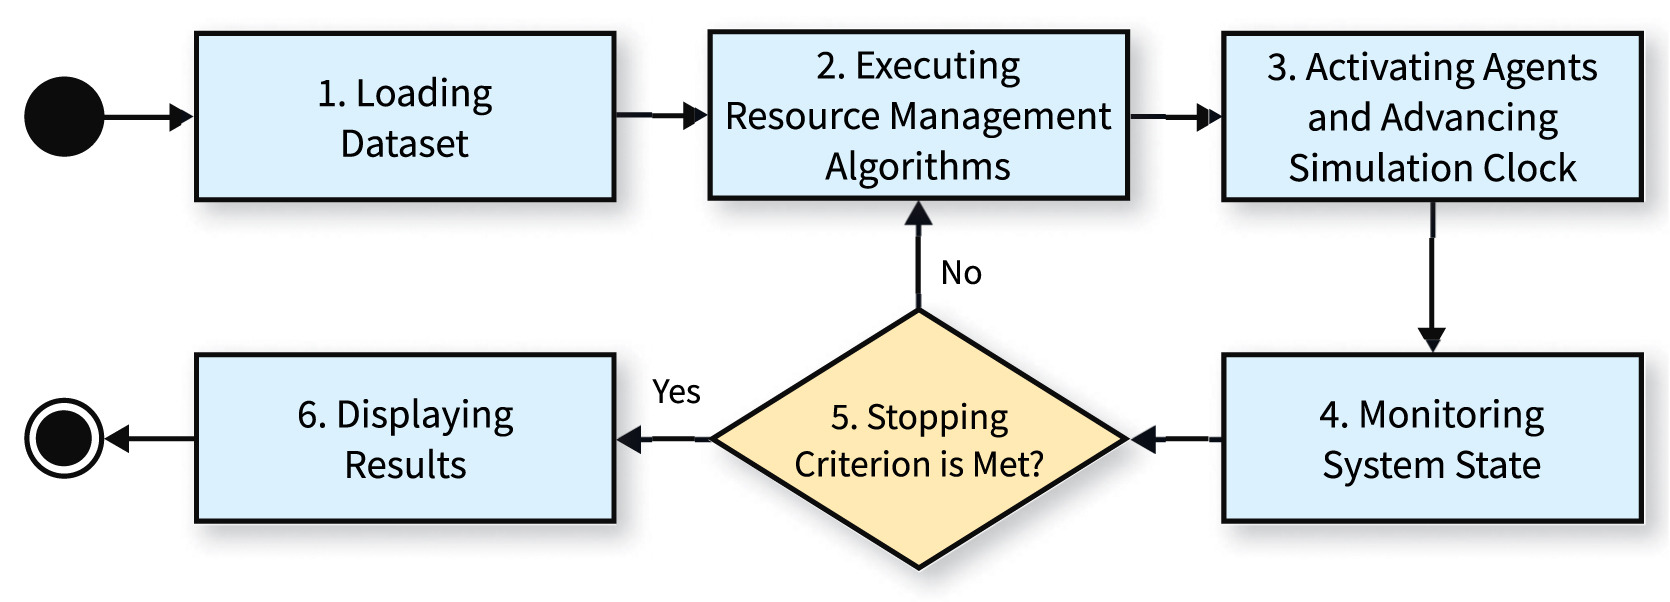
\includegraphics[width=0.75\linewidth]{edgesimpy.jpg}
    \caption{\textit{EdgeSimPy}'s simulation workflow \cite{edgesimpy2023}}
    \label{fig:edgesimpyflow}
\end{figure}

\section{SimPy} \label{SimPy}
The previous section discussed existing simulators that are purpose-built for MEC simulations. They were all designed to address a broad range of issues in the MEC field. However, this meant that implementing simulations that will be in the narrow scope of this project would require significant changes to the existing software. So, a custom-built simulator is needed for this project.

\begin{leftbar}
    SimPy is a process-based discrete-event simulation framework based on standard Python. \cite{simpy2026}
\end{leftbar}

\textit{SimPy} is not a MEC simulator. In fact, it is not a simulator at all. It is a Python framework that can be used to design one's own discrete event simulator (DES), rather than starting from scratch. When working with \textit{discrete events}, this means that the system state changes at discrete points in simulated time. For example, if $time=100$ and the next event is scheduled to occur at $time=150$, then the engine can advance directly to $time=150$ rather than simulating all fifty ticks in between unnecessarily. This is a different, but not mutually exclusive, model to the agent-based simulator in subsection \ref{EdgeSimPy}.

The \textit{SimPy} framework handles things like the simulation clock and event scheduling, but leaves much of the simulator design up to the programmer. The documentation lists example applications of the framework as simulating a \enquote{car wash}, \enquote{gas station refuelling}, a \enquote{machine shop}, and more.

The reuse of existing software is a well-established practice \cite{meyer1997oosc}, allowing developers to avoid unnecessarily reimplementing existing functionality. Accordingly, the development of a custom simulator does not necessarily imply implementing every component from scratch. By using SimPy, the discrete-event simulation functionality can be reused while the computational models and scheduling algorithms specific to this project can be implemented separately.

However, a distinction must be made between extending software through its existing interfaces and modifying its underlying implementation. The Open–Closed Principle \cite{meyer1997oosc} advocates that software entities should be \enquote{open for extension} but \enquote{closed for modification}. Modifying existing code may introduce unintended interactions with other components that depend on their established behaviour. This is why adapting existing simulators' computational models to support the parallel execution of tasks across local, edge, and cloud resources is an issue. By contrast, using SimPy allows the required functionality to be developed through existing interfaces, without altering the underlying discrete-event simulation engine.

\textit{SimPy} allows for the representation of multiple activities happening simultaneously. This is particularly useful for the parallel aspect of this project, which will showcase the speedup of executing some of a task's constituent parts simultaneously versus executing the entire task serially.

The capacity of local processors, edge servers, and the cloud server can all be represented by the \codepill{Resource} class. This comes with request queues and resource allocation mechanisms built in, and will allow for MIPS-based execution of tasks and subtasks.

Another major benefit of \textit{SimPy} for this project is the way it handles process synchronisation. Supposing a task has been divided into one set to be executed locally and one for the edge, the parent process will only resume once all subtasks have finished. This will be important when discussing \textit{synchronisation constraints}, the idea that subtasks have a collective completion time determined by the slowest one (see section \ref{Parallelisable Task Scheduling}). Conceptually, code like this can be written:

\begin{minted}{python3}
local = env.process(execute_locally(125))  # 125 subtasks to execute locally
edge = env.process(execute_on_edge(25))    # 25 to execute on the edge server
yield env.all_of([local, edge])            # resumes when full task is done
\end{minted}

\section{Parallelisable Task Scheduling} \label{Parallelisable Task Scheduling}
The referenced papers in this section (and in Section \ref{Task Offloading Due To Local Constraints}) use slightly different language (such as a \textit{job} being made up of \textit{tasks}), so to avoid confusion this discussion will use a consistent terminology of each \textit{task} being made up of smaller \textit{subtasks}, all of which can be (given sufficient hardware resources) executed in parallel, independently of each other.

The scheduling of parallel subtasks is a research problem that is certainly not unique to the area of edge computing. Shafiee and Ghaderi \cite{shafiee2020parallel} investigated parallel subtask execution internally within one large cluster. An example application they used was \textit{MapReduce}. Each stage (e.g. the \textit{Map} stage) can be thought of as a task, and each worker (e.g. \textit{mapper}) can be thought of as a subtask. The paper designs scheduling algorithms with theoretical guarantees under three main constraints:

\textbf{Packing Constraint:} Each machine can process some number of tasks at the same time. This maps directly to this project, in which there are three \enquote{machines}: a user device, an edge cluster, and the cloud. Each one consists of \textit{processors} that can execute subtasks in parallel

\textbf{Synchronisation Constraint:} Subtasks that belong to the same task have a \enquote{collective completion time}, determined by the slowest subtask. Again, this is applicable to this project, where it will be necessary to compare a task's overall completion time when parallelised against its serial execution.

\textbf{Placement Constraint:} A subtask's execution time is machine-dependent. The speed at which machines in their cluster could read/write to disks depended on proximity. With this project, the RTTs and computational power of each \enquote{machine} represent this same constraint.

Their algorithms prioritise \textit{time} as the variable to be optimised, which seems appropriate to replicate in this project. They consider memory as their 1-dimensional \enquote{resource requirement}. Whilst it is important to reduce multi-dimensional problems down to very few dimensions (by fixing all other parameters) \cite{chipman2021letspracticepreachplanning}, it seems like for this project that \textit{computational demand} would be a more suitable and natural \enquote{resource requirement}.
\newpage
Finally, they describe differences between \textit{preemptive} and \textit{non-preemptive} scheduling. Preemptive scheduling means that a subtask can be paused on a processor. This can be to allow a higher-priority subtask to execute on that processor first and/or to migrate a subtask to another processor. In any case preemption is a prerequisite for mid-execution migration. In non-preemptive scheduling, once a subtask has started execution on one processor, it cannot be paused (and hence, definitely cannot be migrated), and must completely finish before anything else can use that processor. Preemption comes with some overhead. This project should investigate both types when proposing algorithms.

\section{Task Offloading Due To Local Constraints} \label{Task Offloading Due To Local Constraints}
The most commonly investigated issue in MEC has been task offloading \cite{mohammad2023offloading}. However, this is usually in the context of an edge server offloading work to the cloud. There is less literature in the area of offloading from a local device to the edge/cloud, and doing so because of local device constraints. In recent times, local devices have become increasingly more powerful. This means that certain subtasks can be executed locally with acceptable delay. This may save on overall latency despite the fact that edge and cloud servers are still generally much more powerful than local devices, as it can avoid the RTT involved in offloading a subtask.

Gabriel et al. \cite{gabriel2024dag} created an algorithm for scheduling tasks across the local device and an edge server. They used a directed acyclic graph (DAG) to represent dependencies between subtasks. Subtasks that don't have a dependency between them (e.g. tasks 2 and 3 in Figure \ref{fig:dag}) can be executed in parallel, but in general, tasks must wait until their predecessors are completely finished before they can start. Modelling dependencies between subtasks is one of the exceptional deliverables of this project.

\begin{figure}
    \centering
    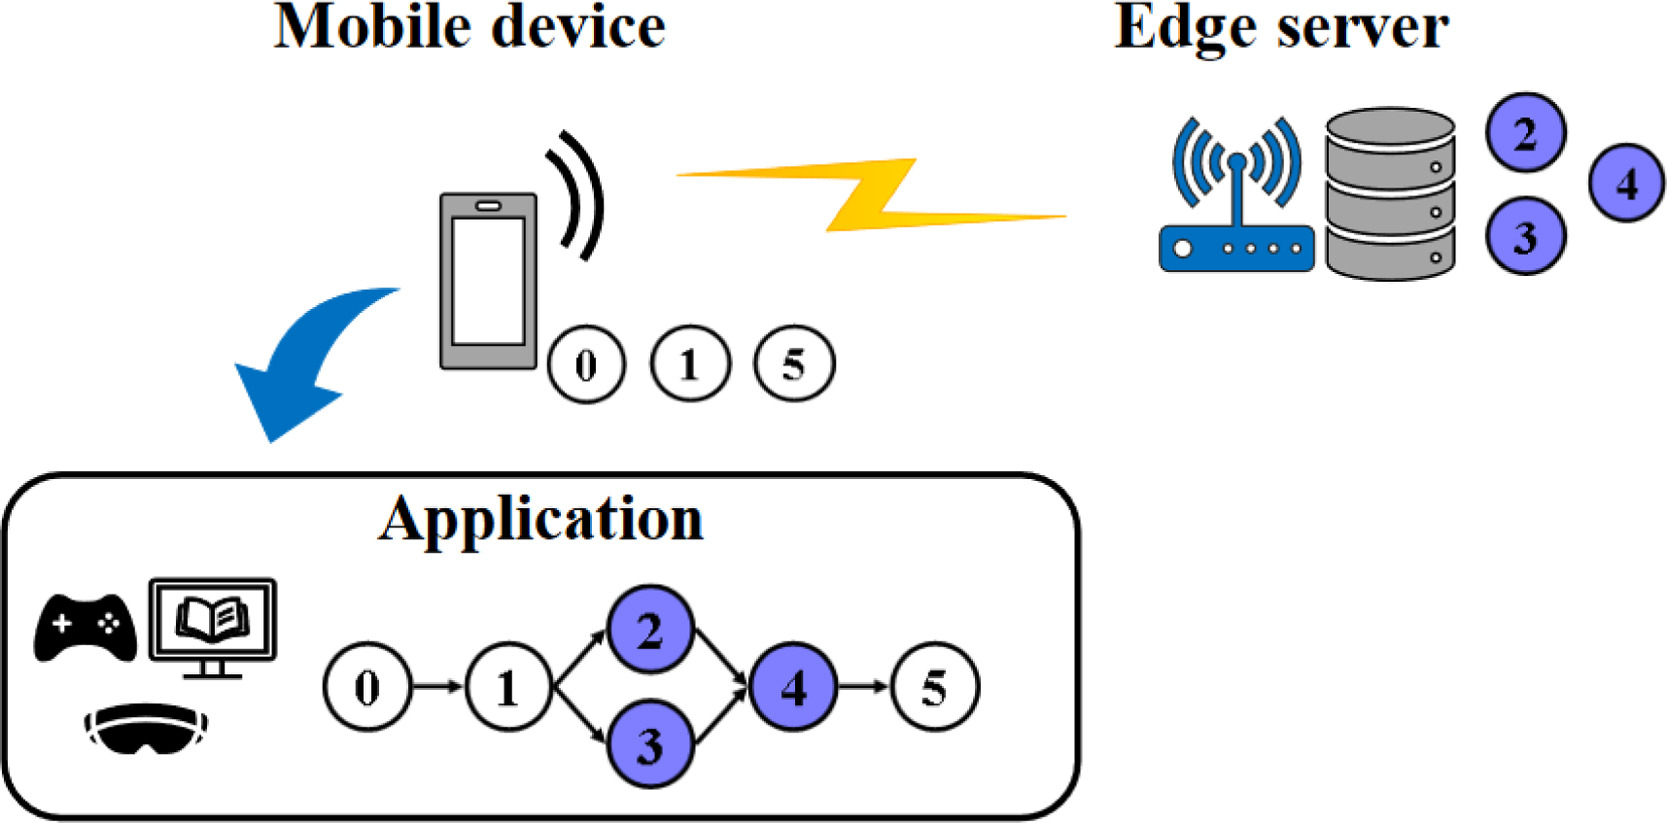
\includegraphics[width=0.5\linewidth]{dag.jpg}
    \caption{DAG representing dependencies between subtasks \cite{gabriel2024dag}}
    \label{fig:dag}
\end{figure}

In their model, every task has a subtask with no incoming edges (the \textit{initial task}) and one with no outgoing edges (the \textit{ending task}). Both must take place on the local device. This is a consideration of realistic parallelisable tasks, where results may need to be combined before presenting a result to the user. This consideration will need to be observed when dependencies are explored.

Time-sharing is used, which significantly complicates latency calculations, while also making offloading decisions much harder since processor speed cannot be trusted. One questionable aspect of their scheduling is that as soon as a subtask is \enquote{ready to start} (i.e. all its predecessors have finished), it is placed onto a processor immediately, regardless of the system state. Considering that every subtask is assumed to be non-preemptive, immediately starting all subtasks means that migration to faster processors is not possible. This wouldn't be a major issue if time-sharing was not used, because the speed of a given processor would instead be fixed. These features will not be applied in this project.

%%%%%%%%
\chapter{Data Considerations}
In this section you should characterise the nature and scale of the data you are working with. Outline the shape of the data, where you expect to obtain it, and the size of the data. Is it static or dynamic, local or remote, stored or streaming? Is it raw or structured? Is it unfiltered user data, or is it curated by a specialist? What is your rationale for using this data and not other data? If your project looks at callout times for Spanish ambulances, usage rates of French parking lots, alcohol consumption in Germany, and so on, then explain why you are not using Irish data for the project. Indicate the data-cleaning processes that you anticipate will be necessary. What licensing restrictions, if any, apply to your data? Will you be making this data public after your project is completed? Are there any privacy or ethical issues with how the data is to be collected or used? If so, discuss here.

Some or many of these questions may be moot in the case of specific projects, but you should provide compelling answers to any that seem relevant. Since this provides the foundation for your project, your reviewers will be looking closely.

%%%%%%%%
\chapter{Outline of Approach}
In this section present an outline of your considered approach to the problem at the centre of your project. Clearly present your design choices, or your choice of algorithms, and any pertinent model parameters. For instance, if you plan to use a genetic algorithm, outline here a sense of your fitness function, major variables, population size, and so on, so that your reviewers can critique your choices. If you opt for a neural architecture, describe your chosen framework, and motivate the number and kinds of layers in your network. In short, be specific about the choices you are committing to at this stage. Being vague and non-specific will not help your case, as your report will be graded in large part on the specificity and perceived wisdom of your choices. Remember also that feedback is intended to help you as you progress to the next stage of your project. If you give reviewers little to chew on, they will not be able to give you specific feedback and guidance.


%%%%%%%%
\chapter{Project Workplan}
In this section you will present a work plan for the remainder of your project. Show that you have considered the issues carefully, and that you can be trusted to lead a research or development effort. Be as specific as you can about the time you expect to allocate to each work component, and the dependencies they have to each other. A Gantt chart is helpful in this respect, but do show some sense in how you present your plan. A naïve understanding makes for a simplistic plan.

A key part of a successful project is evaluation. It is not enough to just state that your project is a success, or that your friends seem to like it. You must have a plan for evaluating the end result. How you evaluate will depend on the nature of your project, and you should have a serious conversation with your supervisor about evaluation before you get to this stage. Will your work yield quantitative results that can be compared to past work or to established benchmarks? Does your work consider different configurations of a system or a solution that you can compare to each other, allowing you to empirically find the best one? Do you have a sample user pool for your planned application, and are they willing to give you structured qualitative and quantitative feedback (e.g. via a questionnaire)? However you plan to evaluate your project, please sketch your intentions here.

%%%%%%%%
\chapter{Summary and Conclusions}
In this section you will sum up your report, draw some conclusions about your work so far, and make some general observations about the work to come. You may also use this opportunity to express points of view, or make factual claims, that are more pertinent here than in other sections of the report. If your project raises some ethical concerns, for example about how data or users are treated, then address them here in a thoughtful manner.

Regarding this document, here are some concluding points that you should keep in mind when writing your own. You may use screenshots in your report, but do not overfill your report with them, or with figures of any kind. Make sure that figures earn their keep, and are not just present as space fillers or as eye candy. If you use diagrams or figures from other people’s work, including the web, be sure to cite the creator in the corresponding caption. All things being equal, it is better to construct your own figures than to copy and paste those of others. In any case, always make sure that your images are readable, do not suffer from pixelation or aliasing effects, and that each is clearly numbered, captioned and meaningfully referenced in the main body of the text.

Ensure that there is a cohesive argument expressed in the text of the report and that it is not simply a bag of diagrams, screenshots and wishful thinking. Every report should tell a story, so know what story you want to tell. When you include images, make sure they are readable and truly add to the discussion.
	
Make sure your language is professional throughout, and steer a course between pompous and colloquial. Maintain authorial distance and do not overuse “me,” “I” and “our.” Your are writing for a professional audience who will judge you on the quality of your prose, so use a grammar and a spelling checker. 

Use LaTeX if you wish – this is recommended if you plan to use mathematical formulae in your report, but in any case, keep the general spacing and font/style you find here (Single or 1.5 spacing, 12 pt. font for text, etc.). Be sure to submit a PDF (never a .DOC or .DOCX file) as your report. If you prepare your report in MS Word, as this document has been, save it as a PDF before you submit it. Overall it should be about 18 – 20 pages, including figures, front matter and references, A significant portion of the report will be textual, with approx.. five or six thousand words. Do not rely on images or other filler to write your report for you. 
The dates and means of submission will be communicated to you separately.


%%%%%%%%%%%%%%%%%%%%%%
%%%% Latex help.
% \chapter{Latex Pointers}

This chapter contains some examples on the usage of latex. Do not include in your final report.

\section{Figures}
From time to time, it's necessary to add pictures to your documents. Using LaTeX all pictures will be indexed automatically and tagged with successive numbers when using the figure environment and the graphicx package. We can reference the figure below using its label like this: Fig. \ref{fig:test_plot}.
\begin{figure}[h]
    \centering
  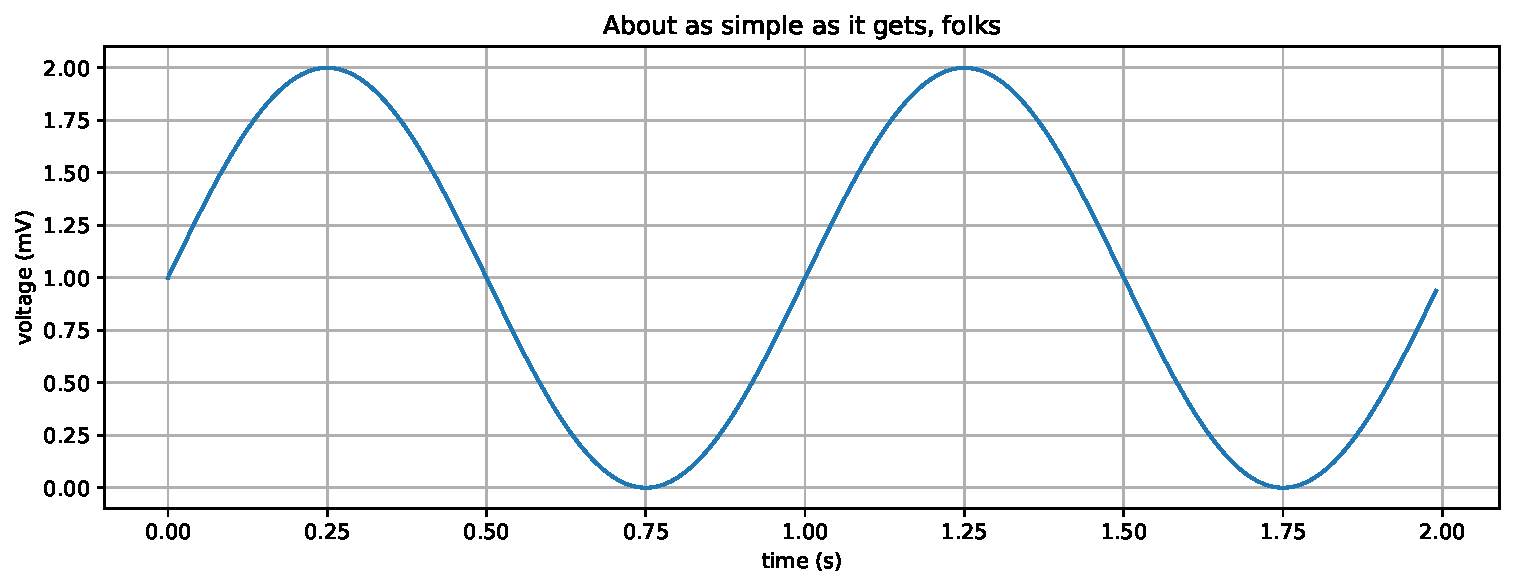
\includegraphics[width=0.8\linewidth]{test_plot.pdf}
  \caption{A sample graph}
  \label{fig:test_plot}
\end{figure}

Lots more information in this \href{https://www.latex-tutorial.com/tutorials/figures/}{tutorial}.


\section{Code Listing}
You can list code using the \emph{listings} package:

\begin{lstlisting}[language=Python,caption=Borg Pattern]
class Borg(object):
    __shared_state = {}

    def __init__(self):
        self.__dict__ = self.__shared_state
        self.state = 'Init'

    def __str__(self):
        return self.state
\end{lstlisting}

Lots more examples \href{https://www.overleaf.com/learn/latex/Code_listing}{here}.

\section{Math}
Here \ref{eq:limit} is an example of including an equation
\begin{equation}
\lim_{x\to\infty} f(x)
\label{eq:limit}
\end{equation}

More examples \href{https://www.latex-tutorial.com/tutorials/amsmath/}{here} and \href{https://www.overleaf.com/learn/latex/Mathematical_expressions}{here}.



\section{References}
Look up the bibtex references on google scholar or import from Mendeley or other reference managers. Add the bibtex snippet to the \emph{references.bib} file. Then cite the reference like this:

As explained in \cite{knuth2014art}, we also find that...

Lots more details \href{https://www.latex-tutorial.com/tutorials/bibtex/}{here}.


%%%%%%%%%%%%%%%%%%%%%%
%%% Acknowledgements
\chapter*{Acknowledgements}
In your Acknowledgements section, give credit to all the people who helped you in your project.


%%%% ADD YOUR BIBLIOGRAPHY HERE
\printbibliography

%%%%
%%%% maybe code listing here?

%%%%
\end{document}
%\end{article}
